\documentclass{article}
\usepackage{graphicx}
\usepackage{subcaption}

\begin{document}
\pagestyle{empty}

\begin{figure}
  \centering
  \begin{subfigure}[t]{0.3\textwidth}
    \centering
    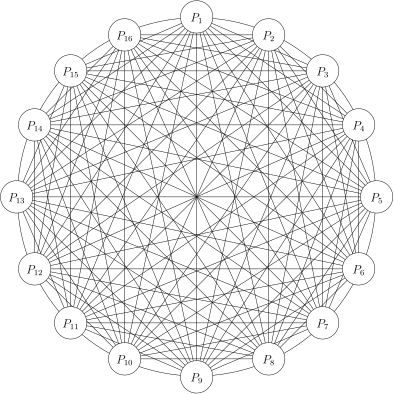
\includegraphics[width=\textwidth]{full-mesh}
    \caption{Full-connected.\newline $\forall P_i, \mathtt{f}[P_i]=T-P_i$.}
    \label{fig:full}
  \end{subfigure}
  \hfill
  \begin{subfigure}[t]{0.3\textwidth}
    \centering
    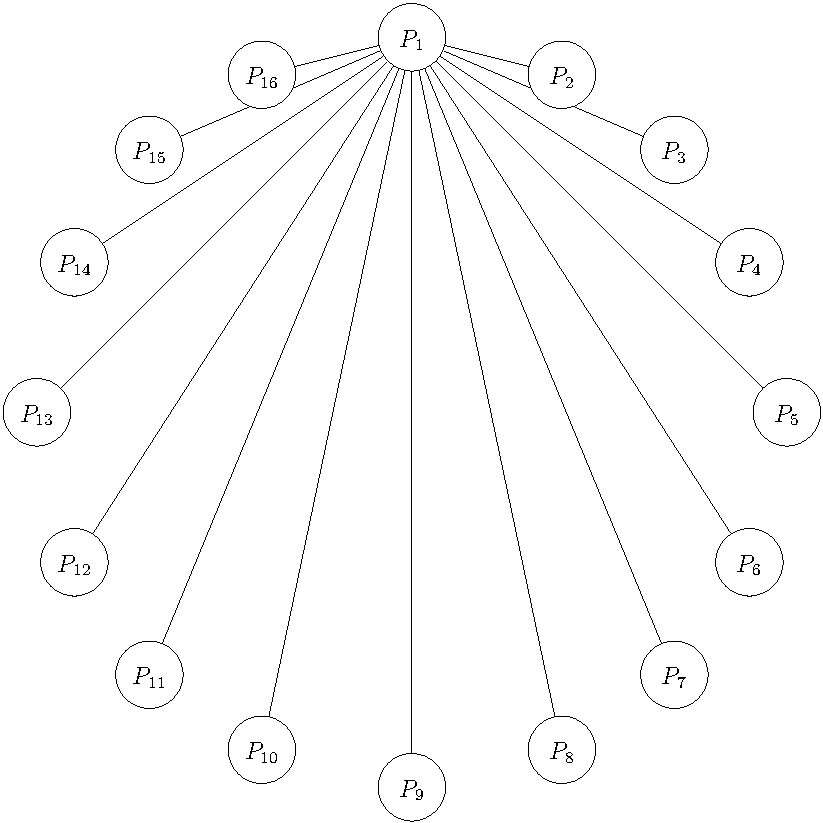
\includegraphics[width=\textwidth]{star}
    \caption{Star-shaped.  \newline $\begin{array}{l} \mbox{In $P_1$}, \mathtt{f}[*] = T-P_1; \\ \mbox{$\forall P_i\neq P_1$}, \mathtt{f}[P_i] = P_1. \end{array}$}
    \label{fig:star}
  \end{subfigure}
  \hfill
  \begin{subfigure}[t]{0.3\textwidth}
    \centering
    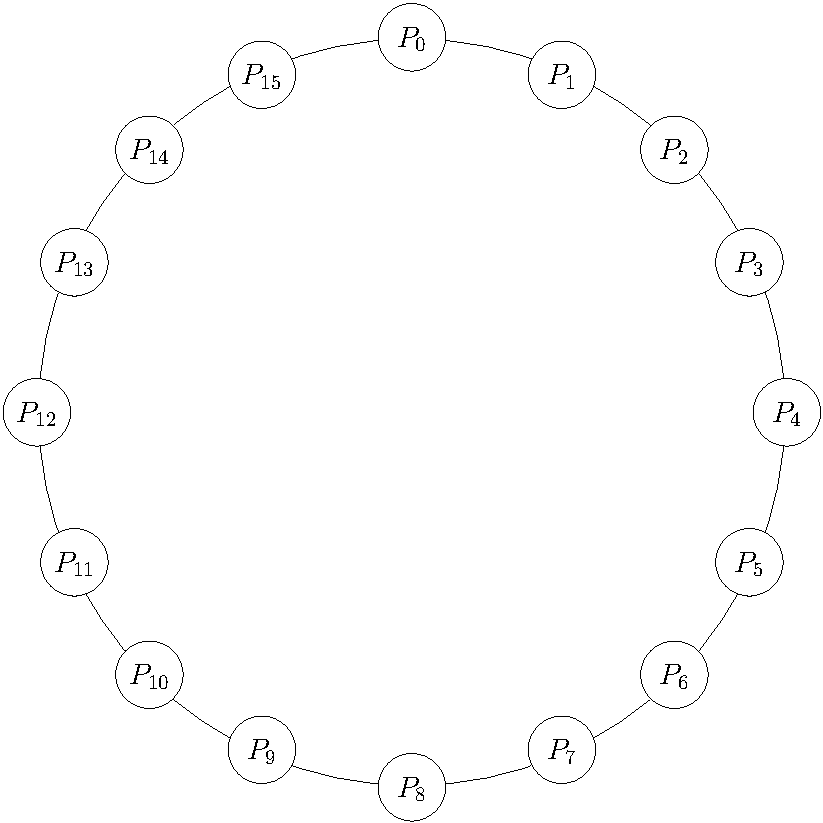
\includegraphics[width=\textwidth]{ring}
    \caption{Ring-shaped. \newline $\forall P_i, \mathtt{f}[P_i]=P_{(i+1)\%N}$.}
    \label{fig:ring}
  \end{subfigure}
\end{figure}%

\end{document}
